
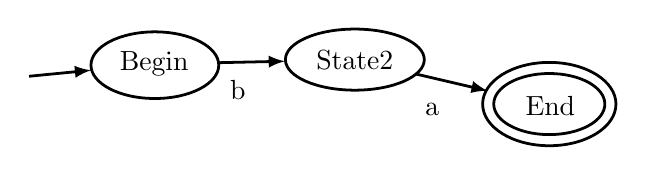
\begin{tikzpicture}[>=latex,line join=bevel,]
  \pgfsetlinewidth{1bp}
%%
\pgfsetcolor{black}
  % Edge: Begin__precursor__ -> Begin
  \draw [->] (54.718bp,26.009bp) .. controls (58.728bp,26.399bp) and (62.901bp,26.804bp)  .. (77.013bp,28.176bp);
  % Edge: State2 -> End
  \draw [->] (193.85bp,26.846bp) .. controls (198.87bp,25.673bp) and (204.31bp,24.4bp)  .. (219.76bp,20.787bp);
  \definecolor{strokecol}{rgb}{0.0,0.0,0.0};
  \pgfsetstrokecolor{strokecol}
  \draw (199.76bp,13.996bp) node {a};
  % Edge: Begin -> State2
  \draw [->] (123bp,30.894bp) .. controls (127.39bp,30.99bp) and (132.06bp,31.093bp)  .. (146.77bp,31.415bp);
  \draw (129.86bp,21.044bp) node {b};
  % Node: State2
\begin{scope}
  \definecolor{strokecol}{rgb}{0.0,0.0,0.0};
  \pgfsetstrokecolor{strokecol}
  \draw (172bp,32bp) ellipse (25bp and 11bp);
  \draw (171.97bp,31.966bp) node {State2};
\end{scope}
  % Node: Begin
\begin{scope}
  \definecolor{strokecol}{rgb}{0.0,0.0,0.0};
  \pgfsetstrokecolor{strokecol}
  \draw (100bp,30bp) ellipse (23bp and 12bp);
  \draw (99.754bp,30.385bp) node {Begin};
\end{scope}
  % Node: End
\begin{scope}
  \definecolor{strokecol}{rgb}{0.0,0.0,0.0};
  \pgfsetstrokecolor{strokecol}
  \draw (242bp,16bp) ellipse (20bp and 11bp);
  \draw (242bp,16bp) ellipse (24bp and 15bp);
  \draw (242.36bp,15.5bp) node {End};
\end{scope}
%
\end{tikzpicture}
